\documentclass{article}
\usepackage{graphicx}
\usepackage[margin=0.7in]{geometry}
\usepackage[T1]{fontenc}
\usepackage[default]{cantarell}
\usepackage{listings}
\usepackage{color}
\usepackage{multicol}
\usepackage{textcomp}
\usepackage[none]{hyphenat}
\usepackage{fancyhdr}
\definecolor{listinggray}{gray}{0.9}
\definecolor{lbcolor}{rgb}{0.94,0.94,0.94}

\begin{document}

\pagestyle{fancy}
\lhead{RobotOpen Control Shield for Arduino v1.0\\Technical Specifications\\www.RobotOpen.biz}
\rhead{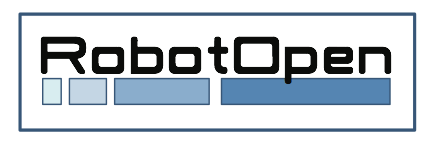
\includegraphics[height=42pt]{robotopen.png}}
\lfoot{www.RobotOpen.biz}
\rfoot{Last Updated January 6th, 2012}
\fancyfoot[C]{}
\setlength\headsep{50pt}
\setlength\footskip{15pt}
\begin{multicols}{2}    % 2 columns


\section*{Overview}
The RobotOpen Control Shield for Arduino is a cRIO drop in replacement for robots. The shield interfaces directly with your FIRST FRC Digital Sidecar. Connection to the sidecar is made over the conventional 37 pin cable. Ethernet is used to interface the controller to an onboard wireless router or network bridge.
\\\\
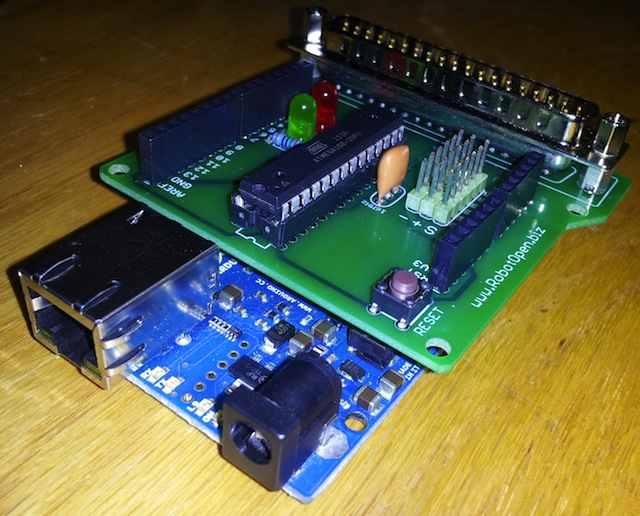
\includegraphics[width=248px]{side.jpg}

\section*{Hardware}

\begin{itemize}

\item 10 PWM (Pulse Width Modulation) channels

\item 8 Digital I/O (can be used as inputs or outputs)

\item Sidecar Pins 5 and 6 can be configured as interrupts

\item 6 ADC (Analog Sensor Inputs)

\item Status indication LEDs and Reset Button

\end{itemize}

\section*{Bundled Software}

\subsection*{Arduino Library}

The RobotOpen Arduino Library makes programming your robots a snap! USB devices connected to your computer are easily accessed through joystick objects in the Arduino environment. Sending data back to your driver station is as simple as calling a single function with the data you'd like to transmit.

\subsection*{Drive Code}

Get your robotics project rolling in minutes. Complete code for Tank Drive, Arcade Drive, and Swerve Drive included. These examples will also bring you up to speed with the RobotOpen Library basics.

\subsection*{Driver Station App}

Connect your joysticks and drive. The included Driver Station app runs on Windows, Mac, or Linux. Logitech and Xbox controller supported out of the box. The application will also display any data you wish to publish from your robot (analog sensors, robot status, etc..) 

\section*{Extensibility}
With RobotOpen we're pushing for openness and extensibility. Our roadmap includes the release of a Java library to ease the creation of your own RobotOpen driver station apps. Don't want to use our library? No problem! Just follow the RobotOpen protocol spec and build your next generation control system from the ground up. Android and iOS based driver station apps are currently in development.
\\\\
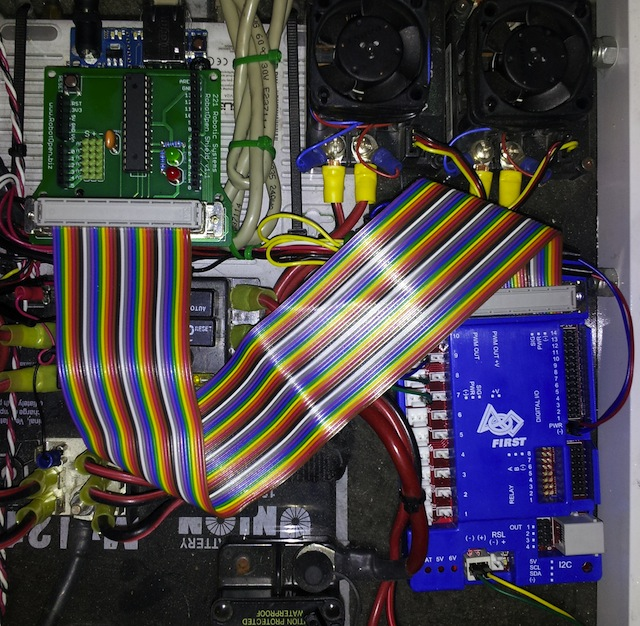
\includegraphics[width=248px]{robot.jpg}

\section*{RobotOpen Protocol}
One of our goals while creating RobotOpen has been to push for a standardized robot control protocol. The RobotOpen protocol is well documented and tested. A few of the features provided by the protocol include:
\begin{itemize}

\item Packetized two-way communication
\item End-to-end integrity verification
\item Arbitrary data transmission
\item Data bundles (grouping of similar data)
\item Low latency (UDP based packets)

\end{itemize}

\end{multicols}

\end{document}  